\chapter{Dimostrazione del teorema della funzione inversa}
\pagestyle{plain}
\thispagestyle{empty}
\pagestyle{fancy}
In questa appendice ci proponiamo di dimostrare in maniera rigorosa il teorema della funzione inversa, riportando tutti i teoremi precedentemente non enunciati necessari per effettuare la dimostrazione. Sarebbe anche interessante mostrare che il teorema del Dini implica il teorema della funzione inversa, mostrando così
che i due teoremi sono equivalenti, tuttavia ciò non verrà fatto.

\begin{theorem}[della funzione inversa]
    Sia $\Omega \subseteq \mathbb{R}^n$ aperto, $f \in C^k(\Omega, \mathbb{R}^n), x_0 \in \Omega$ e $Df(x_0) \in \mathbb{R}^{n \times n}$ invertibile. \\
    Allora $\exists \rho > 0: \exists U \subseteq \mathbb{R}^n$ aperto tali che $f_{|_{B(x_0, \rho)}} \in C^{k}(B(x_0, \rho), U)$ è invertibile e, posto $g=(f_{|_{B(x_0, \rho)}})^{-1}:U \to B(x_0, \rho)$, abbiamo che
    $g \in C^k(U, B(x_0, \rho))$ con
    $$
    Dg(y) = (Df(g(y)))^{-1} \, \forall y \in U
    $$
    \label{thm:inverse_function}
    \end{theorem}

\section{Norma matriciale indotta}

Per dimostrare questo risultato, è conveniente passare ad una norma differente di quella di Hilbert-Schmidt. Sebbene tutte le norme, in uno spazio finito dimensionale sono equivalenti (e dunque inducono la stessa topologia) l'utilizzo di questa norma rende più semplice la trattazione
di alcuni risultati di cui abbiamo bisogno. Iniziamo dando la definizione di spazio delle applicazione lineari fra due spazi vettoriali, la quale dovrebbe già essere stata data nel corso di Geometria, che riporto per completezza
\begin{definition}[spazio delle applicazioni lineari]
    Siano $X, Y$ due spazi vettoriali su un campo $\mathbb{K}$. Definiamo
    $$
    \mathcal{L}(X, Y) = \{f: X \mapsto Y \, | \, f \text{ è lineare} \}
    $$
\end{definition}
\begin{remark}
    Se $A : \mathbb{R}^n \mapsto \mathbb{R}^n$ lineare, scriveremo che $A \in \mathcal{L}(\mathbb{R}^n)$
\end{remark}
\begin{remark}
    $\mathcal{L}(X, Y)$ con $X, Y$ spazi vettoriali su un campo $\mathbb{K}$ è uno spazio vettoriale
\end{remark}
\begin{definition}[norma matriciale indotta]
    Sia $A \in \mathcal{L}(\mathbb{R}^n, \mathbb{R}^m)$, allora definiamo la norma $|| A ||$ matriciale di A come
    \begin{equation}
        || A || = \sup_{x \in \mathbb{S}^{n-1}} |Ax|
    \end{equation}
    dove $|\cdot|:\mathbb{R}^m \to \mathbb{R}$ è la usuale norma euclidea.
\end{definition}
\begin{remark}
    Questa norma viene chiamata, in maniera suggestiva, \emph{indotta} siccome non è altro che la norma vettoriale utilizzata in $\mathbb{R}^n$ che viene "indotta" sullo spazio delle matrici considerando il $\sup$ della norma euclidea della matrice applicata sui vettori di norma $1$.
\end{remark}
\begin{remark}
    Si potrebbero definire le $p-$norme indotte, definite nell'usuale maniera riportata sopra, dove si utilizza come norma vettoriale la norma $|| \cdot ||_p \, : \mathbb{R}^n \to \mathbb{R}$ tale che
    $$
    (x_1, \ldots, x_n) \stackrel{||\cdot||_p}{\mapsto} \left( \sum_{i=1}^n |x_i|^p \right)^{\frac{1}{p}}
    $$
\end{remark}
\begin{remark}
    Osserviamo che
    \begin{equation}
    |Ax| \leq || A || \, |x|
    \label{eq:matrix_norm_inequality}
    \end{equation}
    vale $\forall x \in \mathbb{R}^n$. Inoltre, se $\exists \lambda \in \mathbb{R} : \forall x \in \mathbb{R}^n, |Ax| \leq \lambda |x|$ allora $|| A || \leq \lambda$
\end{remark}
\begin{exercise}
    Mostrare la disuguaglianza (\ref{eq:matrix_norm_inequality}).
\end{exercise}
\begin{proof}[Svolgimento]
    Sia $x \in \mathbb{R}^n$. Allora sappiamo che
    $$
    |Ax| = \big|A( \, |x| \, \frac{x}{|x|} )\big| = |x| \, \big|A\frac{x}{|x|}\big| \leq |x| \, || A ||
    $$
    siccome $\frac{x}{|x|}$ è un vettore di norma unitaria.
\end{proof}
Per pura completezza, riporto la dimostrazione che due norme, nel caso finito-dimensionale, sono \emph{equivalenti}
\begin{definition}[equivalenza fra norme]
    Sia $V$ un $\mathbb{K}-$spazio vettoriale e siano $||\cdot||_1, ||\cdot||_2$ due norme definite sullo spazio vettoriale. Allora diremo che esse sono equivalenti se esistono due costanti $c$ e $C$ strettamente positive per cui
    \begin{equation}
        \forall x \in V, c||x||_1 \leq ||x||_2 \leq C||x||_1.
    \end{equation}
\end{definition}
\begin{remark}
    Due norme equivalenti inducono la stessa topologia (impropriamente la stessa metrica), quindi strutture topologiche quali gli insiemi aperti, le funzioni continue e successioni convergenti rimarrano tali "cambiando" norma: questo potrà sembrare di poco conto e un'astrazione non necessaria, tuttavia, ripensando a come abbiamo costruito tutta la teoria dei limiti e delle successioni in $\mathbb{R}^n$, ci accorgiamo che la norma è l'oggetto su cui abbiamo basato la nostra nozione di convergenza. Dire che
    due norme inducono la stessa topologia vuol dire che presi due oggetti $x, y \in \mathbb{R}^n$ tali che $|x - y| \to 0$ (dove con $|\cdot|: \mathbb{R}^n \to \mathbb{R}$ intendo la norma euclidea) allora presa una qualunque altra norma $||\cdot||_{\star}: \mathbb{R}^n \to \mathbb{R}$ avremo che $||x - y||_{\star} \to 0$. 
    Questo è un risultato non banale e che, in generale, non è vero per spazi vettoriali infinito-dimensionali.
\end{remark}
\begin{prop}[tutte le norme sono equivalenti a quella euclidea su $\mathbb{R}^n / \, \mathbb{C}^n$]
    Sia $n \in \mathbb{N}$. Tutte le norme su $\mathbb{R}^n$ (o $\mathbb{C}^n$) sono equivalenti alla norma euclidea.
    \label{thm:equiv_norme_euclidea}
\end{prop}
\begin{proof}
    Senza perdita di generalità effettueremo la dimostrazione nel caso di $\mathbb{R}^n$. Sia $|| \cdot ||_{\star}$ una norma su $\mathbb{R}^n$ e denotiamo con $||x||_2$ la norma euclidea. Siano $\{e_1, \ldots, e_n \}$ una base canonica su $\mathbb{R}^n$, allora $\forall x \in \mathbb{R}^n, \exists x_1, x_2, \ldots, x_n \in \mathbb{R}^n : x = x_1 e_1 + \ldots + x_n e_n;$ possiamo allora
    applicare ripetutamente la disuguaglianza triangolare sulla norma di $x$ per minorarla
    $$
    ||x||_{\star} = ||\sum_{i=1}^n x_i e_i ||_{\star} \leq \sum_{i=1}^n ||x_i e_i||_{\star} = \sum_{i=1}^n |x_i| ||e_i||_{\star} \leq \sqrt{\sum_{i=1} |x_i|^2 \sum_{i=1}^n ||e_i||^2_{\star}} = ||x||_2 \sqrt{\sum_{i=1}^n ||e_i||^2_{\star}}.
    $$
    dove nell'ultima minorazione si è utilizzata la disuguaglianza di Cauchy-Schwarz. \\
    Dunque se poniamo $A = \sqrt{\sum\limits_{i=1}^n ||e_i||^2_{\star}}$ otteniamo che $||x||_{\star} \leq A||x||_2 \, \, \forall x \in \mathbb{R}^n$, ovvero la norma euclidea domina la norma $\star$. A questo punto, per vedere che la norma $\star$ domina quella euclidea, possiamo considerare la funzione
    $$
    f(x) = ||x||_{\star}
    $$
    Osserviamo che
    $$
    |f(x) - f(y)| = | \, ||x||_{\star} - ||y||_{\star}| \leq ||x-y||_{\star} \leq A||x-y||_2, \, \, \forall x, y \in \mathbb{R}^n,
    $$
    questo prova che la funzione $f$ è lipschtziana, dunque continua rispetto alla norma euclidea. Consideriamo la sfera unitaria $\mathbb{S}^{n-1}$: tale insieme è infatti compatto per il teorema di Heine-Borel (teorema \ref{thm:heine_borel}) in quanto limitato (banale) e chiuso (corollario del lemma \ref{lemma:frontiera_chiusa} dimostrato più avanti), conseguentemente, avremo per il teorema di Weierstrass (teorema \ref{thm:weierstrass}) che 
    la funzione $f$ assumerà massimo e minimo. Sia $u_{\star} \in \mathbb{S}^{n-1}$ tale che
    $$
        \min_{u \in \mathbb{S}^{n-1}} ||u||_{\star} = \min_{u \in U} f(u) = f(u_{\star}) = ||u_{\star}||_{\star}.
    $$
    Indichiamo tale risultato con $B = ||u_{\star}||_{\star} > 0$ è strettamente positivo siccome $||v||_{\star} = 0 \iff v = 0$ (una delle proprietà di cui gode la norma) e nel nostro caso stiamo considerando $u \in \mathbb{S}^{n-1} = {u \in \mathbb{R}^n : ||u||_2 = 1}$, dunque $\forall u \in \mathbb{S}^{n-1}, u \neq 0$. Ma allora, per ogni $x$ non nullo abbiamo che
    $$
    ||x||_{\star} = || \, ||x||_2 \, \frac{x}{||x||_2} \, ||_{\star} = ||x||_2 \, || \, \frac{x}{||x||_2} \, ||_{\star} \geq ||x||_2 \, B
    $$
    siccome $\frac{x}{||x||_2}$ è un vettore unitario rispetto alla norma euclidea e, per quanto visto prima, abbiamo che $\forall u \in \mathbb{S}^{n-1}, B = ||u_{\star}||_{\star} \leq ||u||_{\star}$, giustificando così la maggiorazione effettuata nell'ultimo passaggio. Concludendo, abbiamo che
    $$
        B |||x||_2 \leq ||x||_{\star} \leq A ||x||_2
    $$
    e
    $$
        \frac{1}{A} ||x||_{\star} \leq ||x||_2 \leq \frac{1}{B} ||x||_{\star}
    $$
    dunque $||\cdot||_{\star}$ e $||\cdot||_2$ sono equivalenti.
\end{proof}
\begin{cor}[tutte le norme sono equivalenti in $\mathbb{R}^n / \, \mathbb{C}^n$]
    Sia $n \in \mathbb{N}$. Tutte le norme sono equivalenti in $\mathbb{R}^n / \, \mathbb{C}^n$.
\end{cor}
\begin{proof}
    Come visto nella dimostrazione del teorema \ref{thm:equiv_norme_euclidea}, sappiamo che prese due norme $||\cdot||_{\star}$ e $||\cdot||_{\ast}$ avremo che $\exists A_{\star}, B_{\star}, A_{\ast}, B_{\ast} \in \mathbb{R}$ tali che
    \begin{align*}
        &B_{\star} \, ||x||_2 \leq ||x||_{\star} \leq A_{\star} \, ||x||_2 & &B_{\ast} \, ||x||_2 \leq ||x||_{\ast} \leq A_{\ast} \, ||x||_2 \\
        &\frac{1}{A_{\star}} \, ||x||_{\star} \leq ||x||_{2} \leq \frac{1}{B_{\star}} ||x||_{\star} & &\frac{1}{A_{\ast}} \, ||x||_{\ast} \leq ||x||_{2} \leq \frac{1}{B_{\ast}} ||x||_{\ast}
    \end{align*}
    pertanto abbiamo che
    $$
    ||x||_{\ast} \leq  A_{\ast} \, ||x||_2 = \frac{A_{\ast}}{B_{\star}} B_{\star} \, ||x||_2 \leq \frac{A_{\ast}}{B_{\star}} \, ||x||_{\star} \implies ||x||_{\ast} \leq \frac{A_{\ast}}{B_{\star}} \, ||x||_{\star}
    $$
    e similmente possiamo vedere che
    $$
    ||x||_{\ast} \geq B_{\ast} ||x||_2 = B_{\ast} \frac{1}{A_{\star}} ||x||_{\star} \implies ||x||_{\ast} \geq \frac{B_{\ast}}{A_{\star}} ||x||_{\star}.
    $$
    Conseguentemente, si conclude che
    $$
    \frac{B_{\ast}}{A_{\star}} \, ||x||_{\star} \leq ||x||_{\ast} \leq \frac{A_{\ast}}{B_{\star}} \, ||x||_{\star},
    $$
    e
    $$
    \frac{B_{\star}}{A_{\ast}} \, ||x||_{\ast} \leq ||x||_{\star} \leq \frac{A_{\star}}{B_{\ast}} \, ||x||_{\ast}.
    $$
    Dunque le norme $||\cdot||_{\star}$ e $||\cdot||_{\ast}$ sono equivalenti.
\end{proof}
\begin{cor}[tutte le norme sono equivalenti su spazi di dimensione finita]
    Sia $V$ un $\mathbb{R}-$spazio (o un $\mathbb{C}-$spazio) di dimensione finita $n$. Allora tutte le norme sono equivalenti. 
    \label{cor:equivalence_norms}
\end{cor}
\begin{proof}
    Senza perdita di generalità faremo la dimostrazione nel caso di $\mathbb{R}-$spazio vettoriale. Sia $(V, ||\cdot||_V)$ uno spazio vettoriale normato reale di dimensione finita $n$ e fissiamo una base $\mathcal{B} = \{ v_1, \ldots, v_n \}$ di tale spazio.
    Sappiamo allora che $\forall v \in V \exists \lambda \in \mathbb{R}^n : v = \sum_{i=1}^n b_i v_i$ con $\lambda = (\lambda_1, \ldots, \lambda_n)$: possiamo dunque considerare l'isomorfismo lineare
    \begin{align*}
        &\phi: \mathbb{R}^n \to V \, \, \text{tale che} \, \, \lambda \in \mathbb{R}^n \stackrel{\phi}{\mapsto} \sum_{i=1}^n \lambda_i v_i \in V.
    \end{align*}
    Grazie a questo isomorfismo possiamo far corrispondere alla norma di $V$ una norma definita su $\mathbb{R}^n$ definita come
    $$
    ||\lambda||_{\star} = ||\phi(\lambda)||_V, \, \, \forall \lambda \in \mathbb{R}^n.
    $$
    Verifichiamo che essa è una norma su $\mathbb{R}^n$: abbiamo che $\phi(\lambda) = 0_V \iff \lambda = \underline{0}$ (siccome $\phi$ è un isomorfismo lineare) e per proprietà della norma $||\cdot||_V$ abbiamo che $||v||_V = 0 \iff v = 0$, dunque abbiamo effettivamente che $||\lambda||_{\star} = 0 \iff \lambda = \underline{0}$. Preso adesso uno scalare $c \in \mathbb{R}$ e $\lambda \in \mathbb{R}^n$, abbiamo che
    $\phi(c\lambda) = c\phi(\lambda)$ (sempre perché $\phi$ è un isomorfismo lineare) e, per proprietà di omogeneità della norma, abbiamo che $||c\lambda||_{\star} = ||\phi(c\lambda)||_V = ||c \phi(\lambda) ||_V = |c| \, ||\phi(\lambda)||_V = |c| \, ||\lambda||_{\star}$, mentre per la disuguaglianza triangolare abbiamo che presi $\lambda_1, \lambda_2 \in \mathbb{R}^n$ abbiamo che
    $$
        ||\lambda_1 + \lambda_2||_{\star} = ||\phi(\lambda_1 + \lambda_2)||_V \leq ||\phi(\lambda_1)||_V + ||\phi(\lambda_2)||_V = ||\lambda_1||_{\star} + ||\lambda_2||_{\star},
    $$
    dove nei passaggio abbiamo utilizzato che $\phi(\lambda_1 + \lambda_2) = \phi(\lambda_1) + \phi(\lambda_2)$ (sempre perché $\phi$ è un isomorfismo lineare) e la disuguaglianza triangolare di cui gode la norma $||\cdot||_V$. Dunque la norma definita come
    $$
        ||\lambda||_{\star} = ||\phi(\lambda)||_V
    $$
    è una norma su $\mathbb{R}^n$. \\
    Siano adesso $||\cdot||_{\flat\star} = ||\phi(\cdot)||_{\flat}$ e $||\cdot||_{\sharp\star} = ||\phi(\cdot)||_{\sharp}$ due norme su $\mathbb{R}^n$. Per il corollario \ref{cor:equivalence_norms} abbiamo che
    $$
    \exists A_\flat, B_\flat, A_\sharp, B_\sharp \in \mathbb{R} : \begin{cases}
        A_\flat \, ||\lambda||_{\sharp\star} \leq ||\lambda||_{\flat\star} \leq B_\flat \, ||\lambda||_{\sharp\star} \\
        A_\sharp \, ||\lambda||_{\flat\star} \leq ||\lambda||_{\sharp\star} \leq B_\sharp \, ||\lambda||_{\flat\star}
    \end{cases} \, \, \forall \lambda \in \mathbb{R}^n.
    $$
    Ma siccome $\phi$ è un isomorfismo suriettivo allora avremo che
    $$
    \begin{cases}
        A_\flat \, ||v||_{\sharp} \leq ||v||_{\flat} \leq B_\flat \, ||v||_{\sharp} \\
        A_\sharp \, ||v||_{\flat} \leq ||v||_{\sharp} \leq B_\sharp \, ||v||_{\flat}
    \end{cases} \, \, \forall v \in V,
    $$
    ovvero le norme $||\cdot||_{\flat}$ e $||\cdot||_{\sharp}$ sono equivalenti.
\end{proof}
\section{Alcuni risulti preliminari per la dimostrazione}

Andiamo ad enunciare alcuni risultati di cui abbiamo bisogno per dimostrare quanto ci siamo prefissi all'inizio di questa appendice. Alcuni di essi dovrebbero essere già noti dal corso di Analisi Matematica:
\begin{theorem}[di Banach-Caccioppoli]
	Sia $X$ uno spazio metrico completo e sia $\varphi: X \to X$ una contrazione (ovvero una funzione $L-$lipschtziana con $L < 1$). Allora $\exists ! x \in X : \varphi(x) = x$
\end{theorem}
\begin{proof}
	Sia $(X, d)$ uno spazio metrico completo e sia $x_0 \in X$. Definiamo una successione $\{ x_n \}$ in maniera ricorsiva, imponendo che
	\begin{align*}
		&x_{n+1} = \varphi(x_n) & &(n = 0, 1, \ldots).
	\end{align*}
	La dimostrazione segue in due \emph{step}: la prima consiste nel mostrare l'esistenza di un punto fisso, la seconda l'unicità di tale punto. \\
	\emph{Esistenza}: l'idea è quella di mostrare che questa successione da noi definita è una successione di Cauchy, da cui segue, data la completezza di $X$, che la successione converge a $x \in X$. \\
	Siccome $\varphi$ è una contrazione, allora $\exists c \in \mathbb{R}$ tale che $c < 1$ e $\forall x, y \in X, d(\varphi(x), \varphi(y)) \leq c d(x, y)$. Dunque avremo che
	$$
	d(x_{n+1}, x_n) = d(\varphi(x_n), \varphi(x_{n-1})) \leq c d(x_n, x_{n-1})
	$$
	Procedendo induttivamente (il caso $n=1$ è naturalmente banale) avremo che
	$$
	d(x_{n+1}, x_n) \leq c d(x_n, x_{n-1}) \leq c^n d(x_1, x_0)
	$$
	mentre se prendiamo $n \neq m$ e supponiamo (senza perdere di generalità) che $n > m$ allora
	\begin{align*}
	d(x_n, x_m) &\stackrel{\text{dis. triang.}}{\leq} \sum_{i = m}^{n-1} d(x_i, x_{i+1}) \leq \sum_{i=m}^{n-1} c^{i} d(x_1, x_0) = d(x_1, x_0) \sum_{i=m}^{n+1} c^{i} = \\
	&= d(x_1, x_0) \left( \frac{1-c^{n+1}}{1-c} - \frac{1 - c^{m+1}}{1-c} \right) = \frac{c^{m} - c^{n}}{1-c} d(x_1, x_0).
	\end{align*}
	Ma, siccome $c < 1$, se $m \to +\infty$ e $n > m$ allora quest'ultima quantità tende a $0$, dunque risulta che $\{ x_n \}$ è una successione di Cauchy. Conseguentemente, essendo $X$ completo,
	tale successione converge ad un punto $x \in X$ e, usando la continuità di $\varphi$, abbiamo che
	$$
	x_{k+1} = \varphi(x_k) \implies \lim_{k \to +\infty} x_{k+1} = \lim_{x \to +\infty} \varphi(x_k) \implies x = \varphi(x).
	$$
	\emph{Unicità}: supponiamo per assurdo che esistano due punti fissi, ovvero $\exists x, y \in X, x \neq y : \varphi(x) = x, \varphi(y) = y$. Allora avremo che
	$$
	d(x, y) = d(\varphi(x), \varphi(y)) \leq c d(x, y) \implies d(x, y) \leq c d(x, y) \implies c > 1
	$$
	il che è un assurdo siccome $\varphi$ è una contrazione.
\end{proof}
\begin{theorem}[criterio di Lipschtiz]
	Sia $\Omega \subseteq \mathbb{R}^n$ convesso, $f: \Omega \to \mathbb{R}^m$ una funzione di classe $C^1(\Omega, \mathbb{R}^m)$ e supponiamo che si abbia $L = \sup\limits_{x \in \Omega} ||Df(x)|| < +\infty$. Allora la funzione
	$f$ è $L-$lipschtziana, ossia
	$$
	\forall x, y \in \Omega, |f(x) - f(y)| \leq L|x-y|
	$$
\end{theorem}
\begin{proof}
	Fissiamo $x, x' \in \Omega$, allora consideriamo la funzione $g(t) = f(tx + (1-t)y)$ con $t \in [0, 1]$, pertanto $g: [0, 1] \to \mathbb{R}^m$ ed è anch'essa di classe $C^1$ e si ha che
	$$
	g'(t) = Df(tx + (1-t)y)(x - y)
	$$
	e, dalla formula fondamentale del calcolo integrale, segue che 
	$$
	f(x) - f(y) = g(1) - g(0) = \int_0^1 g'(t)dt = \int_0^1 Df(tx + (1-t)y)(x-y)dt
	$$
	da cui segue che
	\begin{align*}
	|f(x) - f(y)| = |\int_0^1 Df(tx + (1-t)y)(x-y)dt| &\leq \int_0^1 || Df(tx + (1-t)y) || |x-y|dt \leq \\
	&\leq \int_0^1 Ldt |x-y| = L|x-y|
	\end{align*}
\end{proof}
\begin{lemma}
    $\forall n > 0, \forall r > 0, \forall x \in \mathbb{R}^n, B_r(x) \subset \mathbb{R}^n$ sono convesse.
\end{lemma}
\begin{proof}
    Fissiamo $n > 0$, $r > 0$ e $x \in \mathbb{R}^n$. Siano adesso $y, z \in B_r(x)$ e consideriamo il luogo dei punti descritti da
    $$
    \alpha = ty + (1-t)z, \text{ con } t \in [0, 1].
    $$
    Allora
    \begin{align*}
    | \alpha - x | &= |ty + (1-t)z - x| \leq |ty + (1-t)z - tx - (1 - t)x| \leq |ty - tx| + |(1-t)z - (1-t)x| = \\
    &=t \, |y - x| + (1-t) \, |z - x| < tr + (1-t)r = r 
    \end{align*}
\end{proof}
\begin{remark}
    Questa dimostrazione è valida, in realtà, per ogni spazio vettoriale munito di norma. Il fatto che le palle siano convesse non è valido per ogni spazio metrico: un esempio può essere dato da $\mathbb{R}^2$ munito della distanza
    $$
    d((x_1, x_2), (y_1, y_2)) = \sqrt{|x_1 - y_1|} + \sqrt{|x_2 - y_2|}
    $$
    dove la palla centrata in $(0, 0)$ e di raggio $1$ assume la seguente forma
    
    \begin{figure}[H]
        \centering
        \scalebox{1.5}{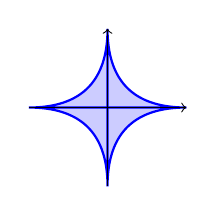
\begin{tikzpicture}
            % Imposta l'area del luogo geometrico
            \fill[blue!20, domain=0:1, samples=200, smooth]
                plot[samples=200, domain=0:1] ({\x^2}, {(1-\x)^2}) -- % Primo quadrante
                plot[samples=200, domain=0:1] ({-(1-\x)^2}, {\x^2}) -- % Secondo quadrante
                plot[samples=200, domain=0:1] ({-\x^2}, {-(1-\x)^2}) -- % Terzo quadrante
                plot[samples=200, domain=0:1] ({(1-\x)^2}, {-\x^2}) -- cycle; % Quarto quadrante
        
            % Disegna il bordo del luogo geometrico
            \draw[thick, blue, smooth, domain=0:1]
                plot[samples=200] ({\x^2}, {(1-\x)^2}) -- % Primo quadrante
                plot[samples=200] ({-(1-\x)^2}, {\x^2}) -- % Secondo quadrante
                plot[samples=200] ({-\x^2}, {-(1-\x)^2}) -- % Terzo quadrante
                plot[samples=200] ({(1-\x)^2}, {-\x^2}) -- cycle; % Quarto quadrante
        
            % Disegna gli assi
            \draw[->] (-1, 0) -- (1, 0);
            \draw[->] (0, -1) -- (0, 1);
        \end{tikzpicture}}
    \end{figure}
\end{remark}
Nel prossimo teorema facciamo uso del seguente risultato che propongo come esercizio
\begin{exercise}
    Sia $A \in \mathcal{L}(\mathbb{R}^n, \mathbb{R}^m)$ e sia $B \in \mathcal{L}(\mathbb{R}^m, \mathbb{R}^k)$, allora
    $$
        || BA || \leq || B || \, || A ||.
    $$
    Mostrare questo risultato sia per la norma matriciale indotta che per la norma di Hilbert-Schmidt
\end{exercise}
\begin{proof}[Svolgimento]
    Nel caso della norma matriciale indotta abbiamo che
    $$
    || BAx || \leq || B(Ax) || \leq || B || |Ax| \leq || B || \, || A || \, |x| \implies || BA || \leq || B || \, || A ||
    $$
    dove abbiamo utilizzato ripetutamente la (\ref{eq:matrix_norm_inequality}). \\
    Per quanto riguarda la norma di Hilbert-Schmidt, osserviamo che, posto $C = BA$, abbiamo che
    \begin{align*}
    || C || = \sqrt{\sum_{i, j} c_{ij}^2} &= \sqrt{\sum_{i}^k \sum_j^n \left( \sum_{k=1} a_{ik} b_{kj} \right)^2} \leq \sqrt{\sum_{i}^k \sum_j^n \sum_{l=1}^m a_{il}^2 \sum_{l=1}^m b_{lj}^2} = \\
    &= \sqrt{\sum_i^k \sum_{l}^m a_{il}^2 \sum_{j}^n \sum_{l}^m b_{lj}^2} = \sqrt{\sum_{i, l} a_{il}^2 \sum_{l, j} b_{lj}^2} = || B || \, || A ||
    \end{align*}
    dove abbiamo utilizzato la disuguaglianza di Cauchy-Schwarz per giustificare la minorazione. Dunque
    $$
    || BA || \leq || B || \, || A ||.
    $$
\end{proof}
\begin{theorem}[continuità dell'operazione di inversione di una matrice]
    Sia $\mathit{\Omega}$ l'insieme di tutte le applicazioni lineari invertibili a valori in $\mathbb{R}^n$. Allora
    \begin{enumerate}[label=\protect\circled{\arabic*}]
        \item Se $A \in \mathit{\Omega}$, $B \in \mathcal{L}(\mathbb{R}^n)$ e
        \begin{equation*}
            || B - A || \cdot || A^{-1} || < 1 \tag{$\ast$}
        \end{equation*}
        allora $B \in \mathit{\Omega}$.
        \item $\mathit{\Omega}$ è un insieme aperto di $\mathcal{L}(R^n)$ e la mappa $A \mapsto A^{-1}$ è continua su $\mathit{\Omega}$ 
    \end{enumerate}
    \label{thm:continuity_of_the_inverse_matrix}
\end{theorem}
\begin{proof}
Mostriamo la \circled{1}. Osserviamo che prese $A \in \mathit{\Omega}, B \in \mathcal{L}(\mathbb{R}^n)$ che soddisfano la ($\ast$) e, per comodità, poniamo $\frac{1}{\alpha} = || A^{-1} ||$ e $|| B - A || = \beta$. Dunque la ($\ast$) diventa
$$
\frac{\beta}{\alpha} < 1 \implies \alpha > \beta.
$$
Osserviamo adesso che $\forall x \in \mathbb{R}^n$
$$
\alpha |x| = \alpha | A^{-1} A x | \leq \alpha || A^{-1} || \, |Ax| = |Ax| = |(A - B + B)x| \leq |(A-B)x| + |Bx| \leq \beta |x| + |Bx|
$$
dunque
\begin{equation*}
0 \leq (\alpha - \beta) |x| \leq |Bx| \tag{\text{$\star$}}
\end{equation*}
dove la prima eguaglianza segue dal fatto che $\alpha - \beta > 0$. Ma questo allora implica che $Bx \neq 0$ se $x \neq \underline{0}$: questo ci permette di concludere, per una serie di noti risultati visti dal corso di Geometria, che $B$ è un isomorfismo, dunque è invertibile, quindi $B \in \mathit{\Omega}$. \\
Mostriamo la \circled{2}. Prendiamo $x = B^{-1}y$ e mettiamola all'interno della ($\star$)
$$
(\alpha - \beta) |B^{-1}y| \leq |BB^{-1}y| = |y|
$$
che una relazione valida $\forall y \in \mathbb{R}^n$ da cui possiamo dedurre che
$$
    |B^{-1}y| \leq \frac{1}{\alpha - \beta} |y| \implies || B || \leq \frac{1}{\alpha - \beta}.
$$
Osservando che
$$
    B^{-1} - A^{-1} = B^{-1} (A-B) A^{-1}
$$
abbiamo che
$$
|| B^{-1} - A^{-1} || \leq || B^{-1} || \, || A - B || \, || A^{-1} || \leq \frac{1}{\alpha - \beta} \frac{\beta}{\alpha} = \frac{\beta}{\alpha (\alpha - \beta)}
$$
e per $\beta \to 0$ osserviamo che $|| B - A || \to 0$, dunque la mappa che associa ad una matrice la sua inversa è continua.
\end{proof}
\begin{remark}
    Il passaggio in cui abbiamo affermato che $|| B || \leq \frac{1}{\alpha - \beta}$ sarebbe fallito con la norma di Hilbert-Schmidt. Sarebbe invece stato corretto nel caso in cui io avessi affermato che $|| B || \leq \frac{\sqrt{N}}{\alpha - \beta}$: il motivo
    di questo deriva dal fatto che in base ortonormale la norma di Hilbert-Schmidt altro non è che $|| B || = \sqrt{\sum\limits_{i=1}^n |Be_i|^2}$ dove $\{e_1, \ldots, e_n \}$ è una qualunque base ortonormale dello spazio vettoriale su cui mi trovo e $|\cdot|:V \to \mathbb{K}$ è la norma su essa definita. Nel caso sopra se risultava che
    $|Bx| \leq \frac{1}{\alpha - \beta} |x| \, \, \forall x \in \mathbb{R}^n \implies |Be_i| < \frac{1}{\alpha - \beta} \implies || B || = \sqrt{\sum\limits_{i=1}^n |Be_i|^2} \leq \sqrt{\sum\limits_{i=1}^n \frac{1}{(\alpha - \beta)^2}} = \frac{\sqrt{N}}{\alpha - \beta}$. Siccome queste dimostrazioni risultano più naturali con la norma matriciale indotta, ho preferito
    passare a questa norma piuttosto che rimanere con quella di Hilbert-Schmidt, sebbene, in linea di principio, queste dimostrazioni si potrebbero "riadattare" siccome le due norme sono equivalenti.
\end{remark}
\begin{lemma}
    $\forall \Omega \subseteq \mathbb{R}^n, \text{Fr} \, \Omega$ è un insieme chiuso.
    \label{lemma:frontiera_chiusa}
\end{lemma}
\begin{proof}
    La dimostrazione è immediata: sappiamo dall'esercizio \ref{exercise:frontiera_intersec} che la frontiera di $\Omega$ è definita come $\text{Fr} \, \Omega = \overline{\Omega} \cap \overline{\Omega^c}$. Conseguentemente,
    abbiamo che $\overline{\Omega}$ è un insieme chiuso, $\overline{\Omega^c}$ è chiuso e abbiamo che
    $$
        (\overline{\Omega} \cap \overline{\Omega^c})^c = (\mathbb{R}^n \setminus \overline{\Omega}) \cup (\mathbb{R}^n \setminus \overline{\Omega^c})
    $$
    ma, per quanto mostrato nella proposizione \ref{prop:set_closed_iff_compl_open}, abbiamo che $\mathbb{R}^n \setminus \overline{\Omega}$ e $\mathbb{R}^n \setminus \overline{\Omega^c}$ sono insiemi aperti e, per quanto visto nell'esercizio \ref{exercise:union_open_set_is_open}, abbiamo che
    l'unione di insiemi aperti è un insieme aperto. Ma allora il complementare di $\text{Fr} \, \Omega$ è aperto, dunque, sempre per la proposizione \ref{prop:set_closed_iff_compl_open}, avremo che è un insieme chiuso.
\end{proof}
\begin{lemma}
    Siano dati $A \subseteq \mathbb{R}^n$ aperto e $B \subseteq \mathbb{R}^n$ chiuso. Allora $A \setminus B$ è aperto e $B \setminus A$ è chiuso.
    \label{lemma:diff_open_closed_set}
\end{lemma}
\begin{proof}
    Siccome $B$ è chiuso, allora $B^c = \mathbb{R}^n \setminus B$ è aperto in virtù della proposizione \ref{prop:set_closed_iff_compl_open}, dunque 
    $$
    A \setminus B = A \cap B^c = A \cap (\mathbb{R}^n \setminus B)
    $$
    tuttavia, per quanto visto nell'esercizio \ref{exercise:intersec_open_set_is_open}, abbiamo che l'intersezione di aperti è un insieme aperto. Per quanto riguarda $B \setminus A$ osserviamo che
    $$
    (B \cap (\mathbb{R}^n \setminus A))^c = B^c \cup (\mathbb{R}^n \setminus A)^c = B^c \cup A
    $$
    che è aperto come conseguenza dell'esercizio \ref{exercise:union_open_set_is_open}, dunque $B \cap (\mathbb{R}^n \setminus A)$ è chiuso sempre per la proposizione \ref{exercise:intersec_open_set_is_open} ma
    $$
    B \setminus A = B \cap (\mathbb{R}^n \setminus A) \implies B \setminus A \text{ è aperto.}
    $$
\end{proof}
\section{Dimostrazione del tereoma}
Procediamo nella dimostrazione del teorema della funzione inversa
\begin{proof}[Dimostrazione (del teorema \ref{thm:inverse_function})]
	Denotiamo con $\mathbb{R}^{n \times n} \ni A = Df(x_0)$. L'idea è quello di utilizzare il teorema di Banach-Caccioppoli per mostrare che, preso un insieme $U \subset f(B(x_0, r))$ aperto sufficientemente piccolo\\
	Siccome $\Omega$ è aperto e $f \in C^1(\Omega, \mathbb{R}^n) \implies Df: \Omega \to \mathbb{R}^n$ è continuo, allora possiamo scegliere $\rho > 0$ in maniera tale che
	\begin{align*}
	&\overline{B_{\rho}(x_0)} \subset \Omega \text{    e    } |Df(x) - Df(x_0)| < \frac{1}{2 || A ||} \forall x \in \overline{B_\rho(x_0)}.
	\end{align*}
	Poniamo $r = \frac{\rho}{2 || A ||}, y_0 = f(x_0)$. Fissato $y \in B_r(y_0)$, consideriamo l'applicazione
	$$
	T : \overline{B_{\rho}(x_0)} \mapsto \mathbb{R}^n \text{ tale che } 	T(x) = x + A(y-f(x))
	$$
	e osserviamo che $T(x) = x \iff y=f(x)$. Allora, ricordando che $ADf(x_0) = \text{Id}$, avremo, per $x \in \overline{B_p(x_0)}$, che
	$$
	|| DT(x) || = || \text{Id} - ADf(x) ||  \leq || A || \, || Df(x) - Df(x_0) || \leq || A || \frac{1}{2 || A ||} = \frac{1}{2}
	$$
	dunque, per il criterio di Lipschtiz, avremo che la funzione $T$ è $\frac{1}{2}-$lipschtziana. Mostriamo adesso che $T(\overline{B_\rho(x_0)}) \subset \overline{B_\rho(x_0)}$: infatti, preso $x \in \overline{B_\rho(x_0)}$, abbiamo che
	\begin{align*}
	|T(x) - x_0| \stackrel{\text{dis. triang.}}{\leq} |T(x) - T(x_0)| + |T(x_0) - x_0| &\leq \frac{1}{2} |x-x_0| + |A(y - y_0)| \leq \frac{\rho}{2} + || A || r = \\
	&=\frac{\rho}{2} + || A || \frac{r}{2 || A ||} = \rho.
	\end{align*}
	Dunque $T : \overline{B_\rho(x_0)} \mapsto \overline{B_\rho(x_0)}$ è una contrazione, $B_\rho(x_0)$ è uno spazio metrico completo (rispetto alla metrica indotta) e, quindi, per il teorema delle contrazioni esiste un'unica soluzione all'equazione
	$$
		T(x) = x.
	$$
	Ma prendendo arbitrariamente $y_0 \in B_\rho(y_0)$ possiamo trovare un unico $x \in B_\rho(x_0)$ che risolve l'equazione $f(x) = y$
	pertanto possiamo definire $g$ l'applicazione $y \in B_{r}(y_0) \mapsto x \in B_{\rho}(x_0)$
	\begin{align*}
		&g: B_{r}(y_0) \subset \overline{B_{\rho} (x_0)} \mapsto \overline{B_\rho(x_0)}, & &f(g(y)) = x.
    \end{align*}
	Cerchiamo di capire, adesso, dove viene mandata la frontiera di $B_\rho(x_0)$. Consideriamo l'insieme $\Sigma = f(\text{Fr} \, B_\rho(x_0))$: dalla continuità di $f$ e dal fatto che $\text{Fr} \, B_\rho(x_0)$ è compatto (è banalmente limitato, è chiuso in virtù del lemma \ref{lemma:frontiera_chiusa} e, dunque, è compatto per il teorema \ref{thm:heine_borel}) deriva che $\Sigma$ è compatto. Inoltre
    $y_0 \neq \Sigma$ siccome, per quanto mostrato in precedenza, $\exists ! x \in \overline{B_\rho(x_0)}$ per cui $f(x) = y_0$ e tale punto è proprio $x_0 \neq \text{Fr} \, B_\rho(x_0)$. Dunque avremo che $V = B_r(y_0) \setminus \Sigma$ è un insieme aperto (in virtù del lemma \ref{lemma:diff_open_closed_set}). Posto $U = g(V)$ risulta che $f_{|U} : U \to V$ è bigettiva
    e ha $g$ come inversa. Inoltre, per costruzione, abbiamo evitato che $U$ possieda tutti i punti di $\text{Fr} \, B_\rho(x_0)$ e, dunque, risulta che $U \subset B_\rho(x_0)$. \\
    Vogliamo mostrare adesso che $U$ è aperto: preso $x \in U$ poniamo $y = f(x)$ da cui, per come abbiamo definito $U$ e $V$, si deduce che $y \in V$. Siccome quest'ultimo insieme è aperto, sappiamo che $\exists \varepsilon > 0: B_\varepsilon(y) \subset V$ ed, essendo $f$ continua, possiamo trovare $\delta > 0$ tale che
    $$
    f(B_\delta(x)) \subset B_\varepsilon(y) \subset V,
    $$
    ma allora, siccome $x \in U \subset B_\rho(x_0)$, a meno di rimpicciolire $\delta$ possiamo supporre che $B_\delta(x) \subset B_\rho(x_0)$. Risulta, dunque, che $f(B_\delta(x)) \subset V \implies B_\delta(x) = g(f(B_\delta(x))) \subset U$. Dunque $U$ contiene un intorno di ogni suo punto, dunque è aperto. \\
    Mostriamo, infine, che $g$ è differenziale in ogni suo punto $y \in B_r(y_0)$ e che il suo differenziale $Dg(y)$ è uguale a $Df(x)^{-1}$ con $x = g(y)$, ossia si vuole mostrare che
    $$
        \lim_{y' \to y} \frac{g(y') - g(y) - Df(x)^{-1}(y'-y)}{|y-y'|} = 0.
    $$
    Osserviamo, tuttavia, che $y \in B_r(y_0)$ dunque stiamo considerando la seguente quantità (che abbiamo riscritto sfruttando la differenziabilità della funzione $f$)
    \begin{align*}
    &\frac{g(y') - g(y) - Df(x)^{-1}(f(x')-f(x))}{|y' - y|} = \frac{x' - x - Df(x)^{-1}(Df(x)(x'-x) + o(|x' - x|))}{|y' - y|} = \\
    &=\frac{Df(x)^{-1}(o(|x'-x|))}{|y'-y|} = \frac{Df(x)^{-1}(o(|x'-x|))}{|x'-x|} \frac{|x'-x|}{|y'-y|}.
    \end{align*}
    Per concludere, ci basta mostrare che se $y' \to y \implies x' \to x$, cosicché il primo termine dell'ultimo prodotto tende a zero per definizione di $o-$piccolo. Per fare questo, possiamo riutilizzare
    l'applicazione $T$ definita in precedenza: ricordando che essa è $\frac{1}{2}-$lipschtziana abbiamo che
    \begin{align*}
    \frac{1}{2} |x' - x| \geq  |T(x') - T(x)| = |x' - x + A(y - f(x))| &\geq |x' - x| - |A(y - f(x'))| = & \\
    &=|x'-x| - || A || \, |y'-y| &
    \end{align*}
    da cui possiamo dedurre che $|x' - x| \leq 2 \, || A || \, |y' - y|$, pertanto $x' \to x$ se $y' \to y$ e per $y' \to y$ il rapporto $\frac{|x'-x|}{|y'-y|}$ è limitato. Questo ci porta a concludere che
    $$
    \frac{Df(x)^{-1}(o(|x'-x|))}{|x'-x|} \frac{|x'-x|}{|y'-y|} \to 0 \text{ per } y' \to y.
    $$
    Questo ci permette di concludere che la funzione $g$ è differenziale in $y$ (e dall'arbitrarietà di tale punto segue che è differenziale per ogni punto in $B_r(y_0)$, dunque anche in $V \subset B_r(y_0)$). A
    questo punto, resta da mostrare che il differenziale $Dg(y)$ è una funzione continua, ma dato che $Dg(y) = Df(g(y))^{-1}$ si osserva che essendo $g$ continua (in quanto differenziabile), essendo $Df$ continua (per ipotesi)
    ed essendo continua anche la mappa che associa ad una matrice la sua inversa (in virtù del teorema \ref{thm:continuity_of_the_inverse_matrix}), la funzione $Dg$ dev'essere continua.
\end{proof}